\section{\review{Dodecapolar Resonance Driving Term}}

% Fill 9339
% https://logbook.cern.ch/elogbook-server#/logbook?logbookId=1081&dateFrom=2024-03-10T00%3A00%3A00&dateTo=2024-03-11T00%3A00%3A00
% http://localhost:8888/lab/workspaces/auto-Z/tree/work_afs2/jupyter/resonance_driving_terms/simulations/first_dodecapole_rdt/Plots.ipynb

During the 2024 commissioning, Resonance Driving Term measurements were conducted by applying
kicks of varying strengths using the AC-Dipole, at injection energy. These measurements aimed to
measure several RDTs, with a particular focus on decapoles and their associated corrections. The
kicks were performed initially with nominal FiDeL settings for the octupolar and decapolar
correctors, followed by additional $Q''$ then $Q''$ and $Q''$ combined corrections.

Thanks to improvements in dynamic aperture resulting from a better understanding of lower-order
multipoles, the high kick amplitudes enabled the observation of a distinct line in the vertical
spectrum at $5Q_y$, as shown in \cref{fig:high_orders:spectrum_dodecapole_5qy}. This line is
attributed to the presence of dodecapolar fields (see \cref{appendix:rdts}) and its amplitude scales
with the vertical action.

\begin{figure}[!htb]
    \centering
    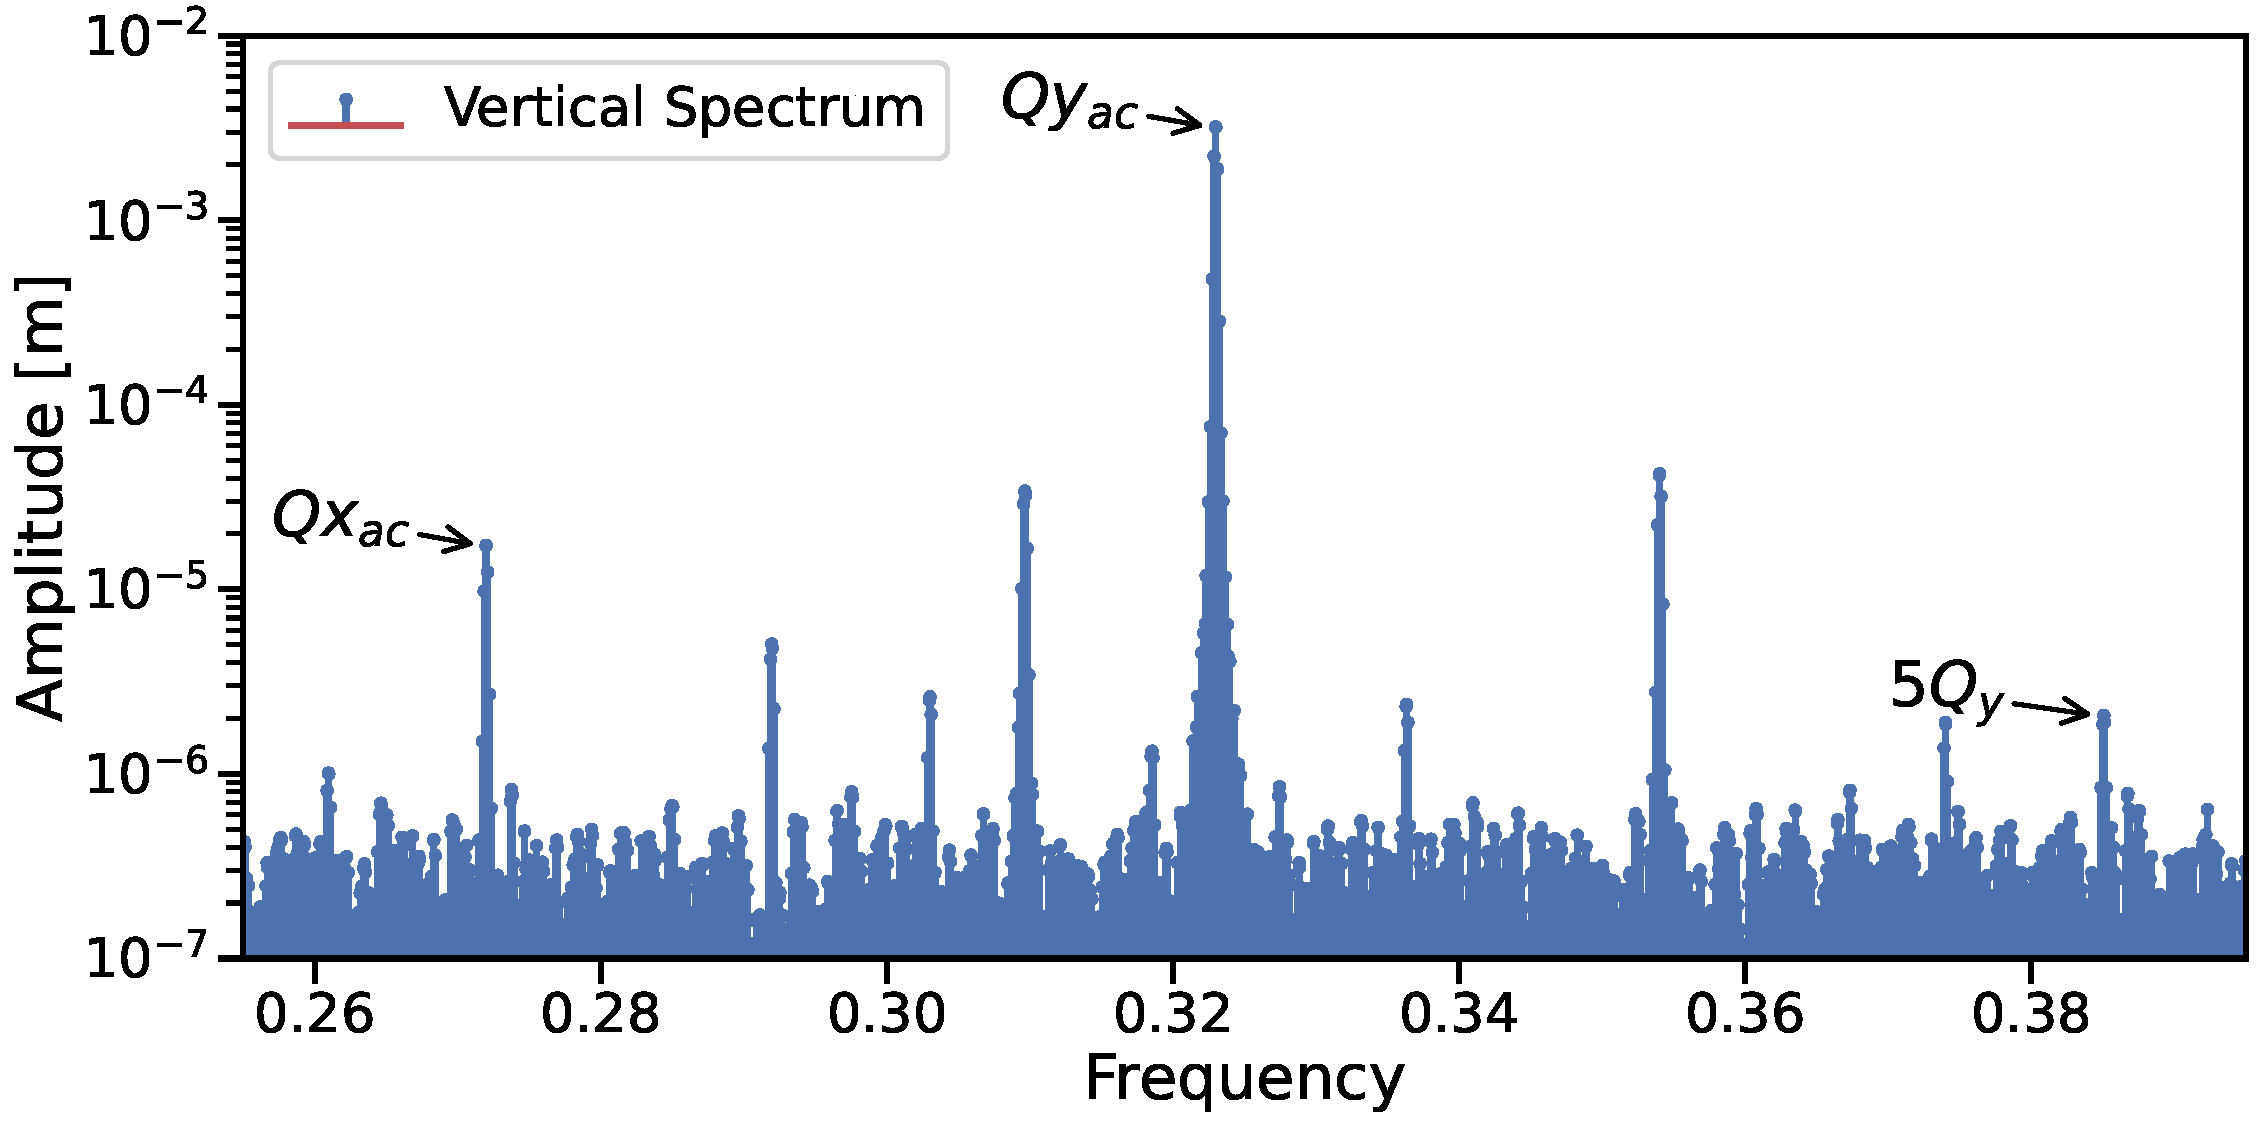
\includegraphics[width=0.8\textwidth]{./images/spectrum_dodecapole_5qy.pdf}
    \caption{Vertical spectrum of recorded turn-by-turn data for Beam 1 showing the tunes driven by
    the AC-Dipole along with a line contributed to by dodecapolar fields.}
    \label{fig:high_orders:spectrum_dodecapole_5qy}
\end{figure}

To achieve these measurements, the kick strength of the AC-Dipole was set up to $40\%$ of its
maximum. The specific excited resonance of the observed line is the $6Q_y$, related to the RDT
$f_{0060}$.
\Cref{fig:high_orders:dodecapolar_f0060} highlights the real part of this RDT taken with nominal
corrections at various kick percentage strengths for a given arc of the LHC.
The clear observation of lines in the frequency spectrum and the agreement between the various
kicks at different actions display the reliability of the measurement.
The RDT reconstructed via the previous kicks is shown in
\cref{fig:high_orders:dodecapolar_f0060_avg}, for which the RMS amplitude is of
$3.5\cdot10^8\;[\text{m}^{-2}]$.

\begin{figure}[!htb]
    \centering
    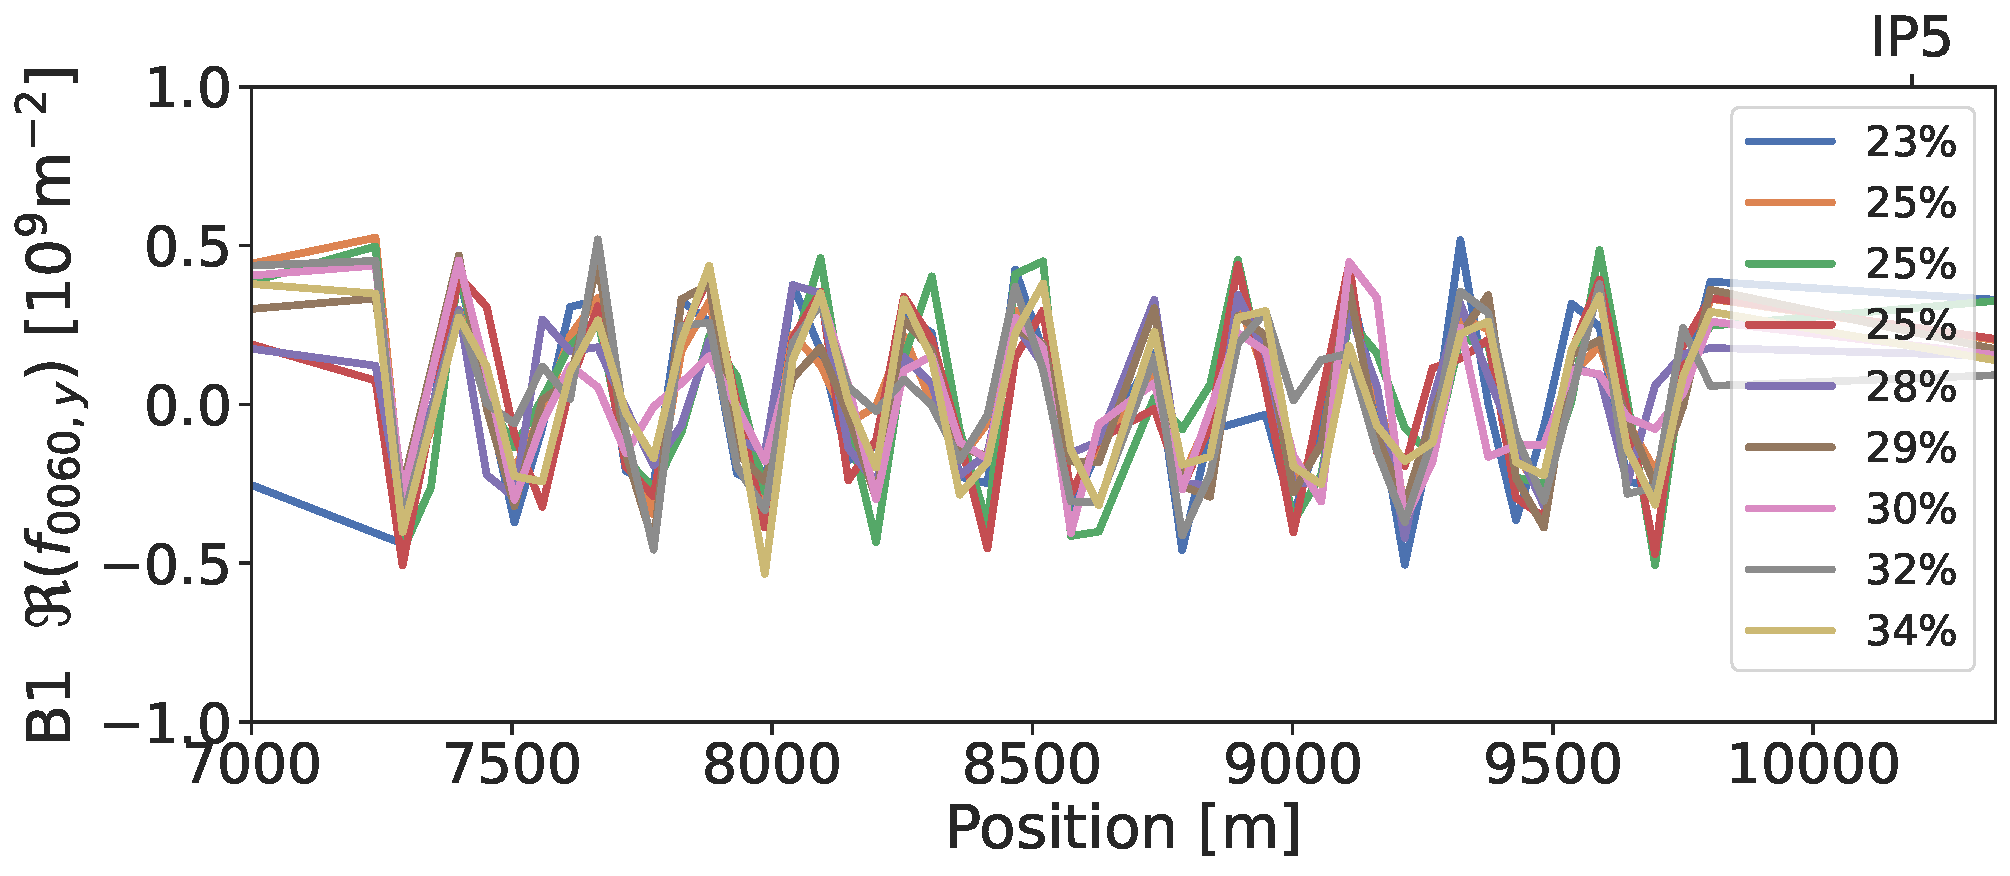
\includegraphics[width=0.8\textwidth]{./images/f0060y_all_meas_real.pdf}
    \caption{Real part of the dodecapolar RDT $f_{0060}$ measured with several kick strengths.}
    \label{fig:high_orders:dodecapolar_f0060}
\end{figure}

\begin{figure}[!htb]
    \centering
    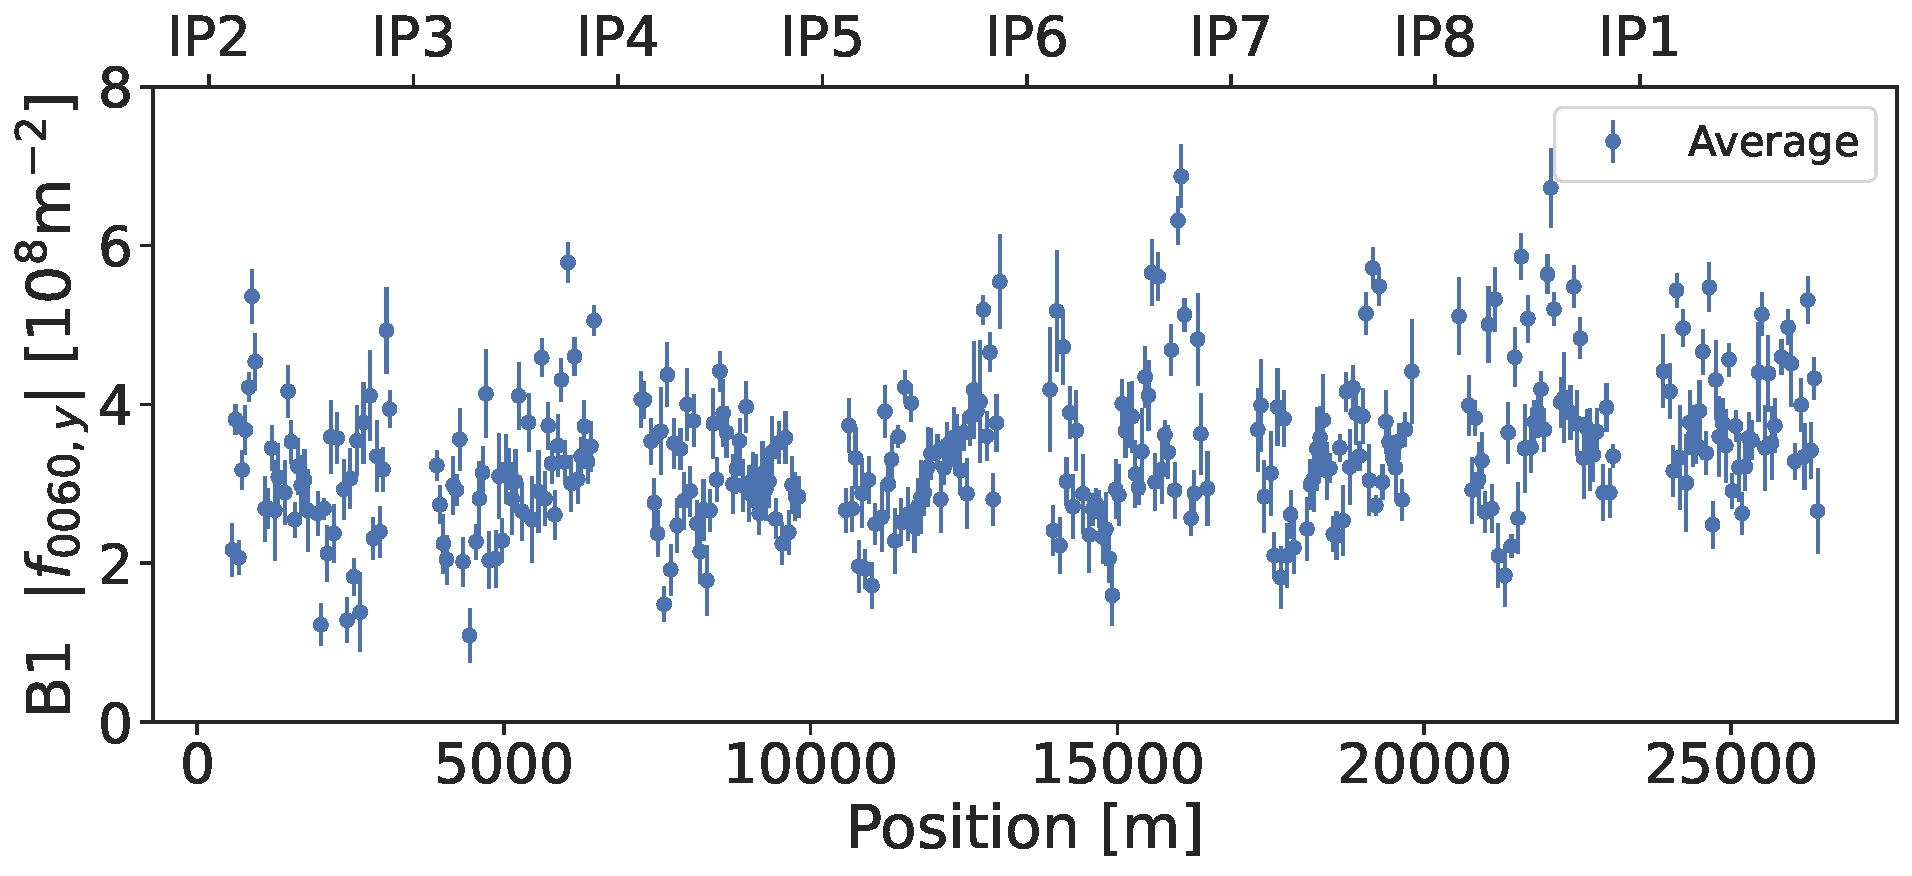
\includegraphics[width=0.8\textwidth]{./images/f0060y_all_meas_avg_amp.pdf} \caption{Amplitude
    of the dodecapolar RDT $f_{0060}$. The RMS amplitude is of $3.5\cdot10^{8}\;[\text{m}^{-2}]$.}
    \label{fig:high_orders:dodecapolar_f0060_avg}
\end{figure}



Similar to the decapoles discussed in \cref{section:decapoles:feed_up}, the dodecapolar RDTs can be
influenced by lower-order components, as shown in
\cref{table:appendix:transfer_maps:bch_resulting_orders_combination}. At the second-order BCH, a
combination of sextupoles and decapoles, as well as a combination of octupoles, generate a
decapolar-like perturbations. At the third and fourth orders, these fields are respectively
generated by a combination of sextupoles with octupoles and by sextupoles.  
Several tracking simulations were performed with various combinations of field errors, ranging from
normal and skew sextupoles ($a,b_3$) to decaoctupoles ($a,b_9$), including as well coupling.
The $b_2$ errors, in the main dipoles and quadrupoles, are not added as they generate a large,
unrealistic, phase error.
\Cref{fig:high_orders:simulations_f0060} shows the RMS amplitude of the RDT $f_{0060}$ for each of
these simulations. As could be expected from the analytical equations, the lower-order multipoles do
contribute to this RDT and seem to cancel the $b_6$ component. It is though apparent that Beam 1 and
Beam 2 do not have the same contributions from the dodecapolar errors. 


\begin{figure}[!htb]
    \centering
    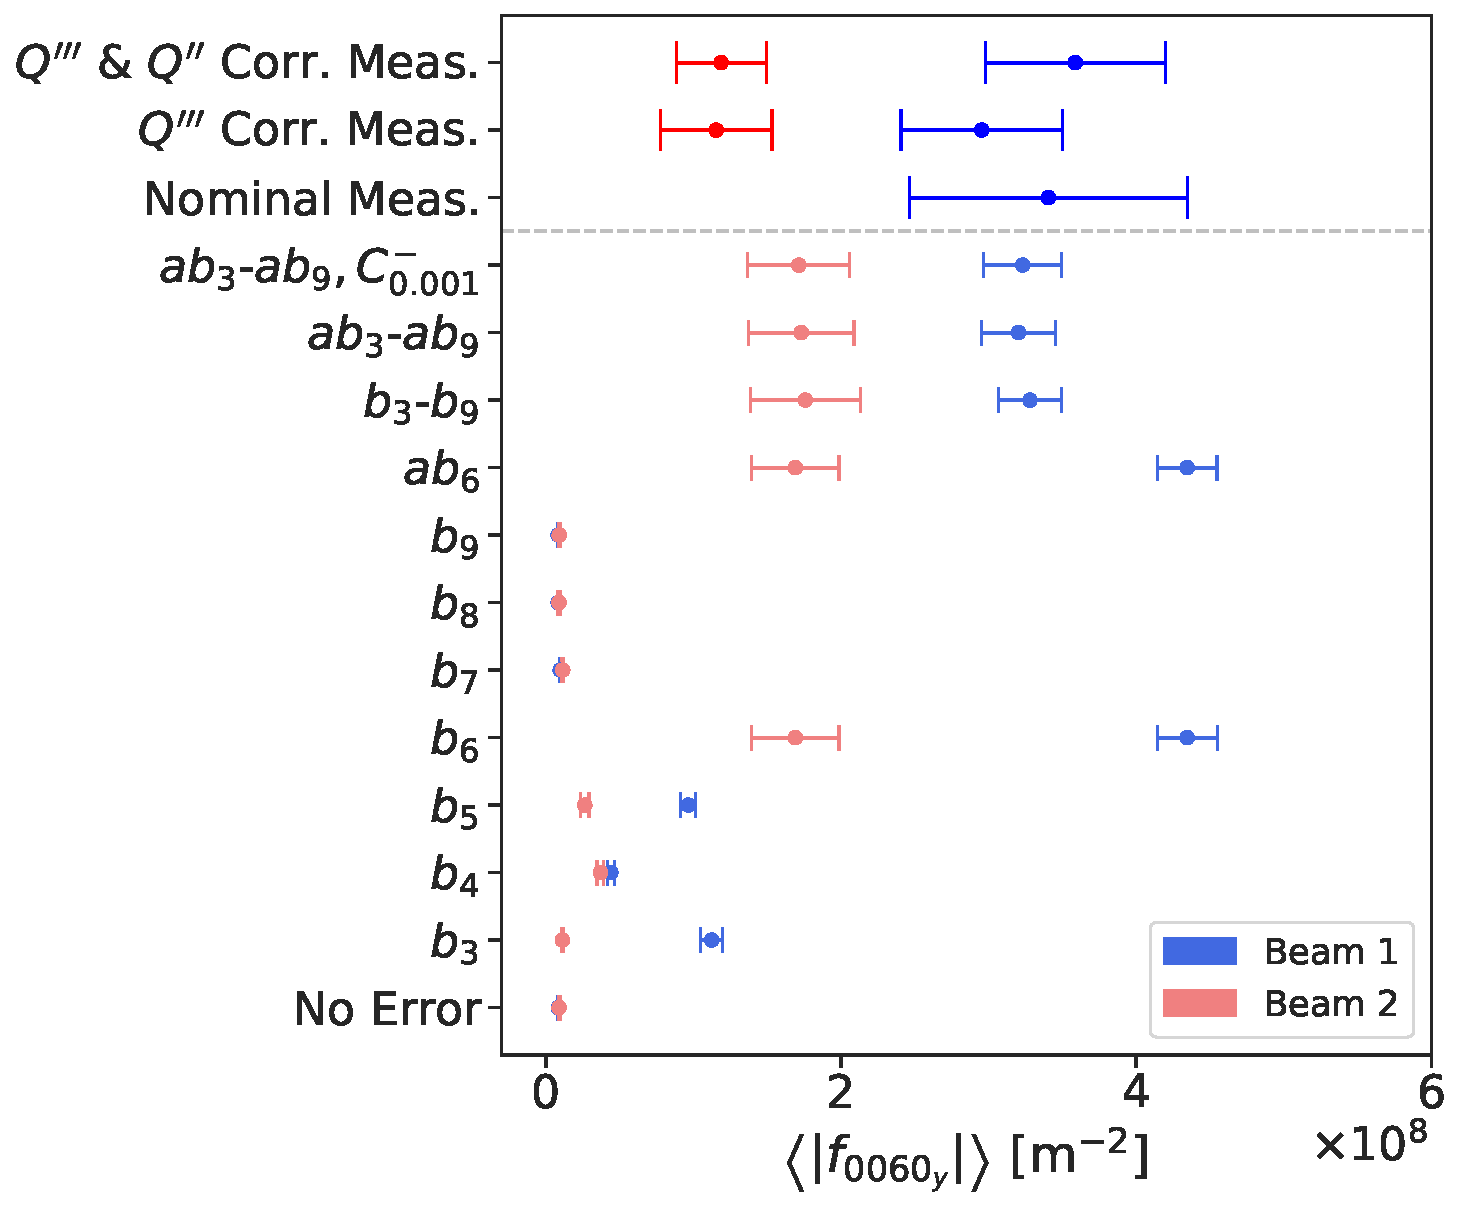
\includegraphics[width=0.7\textwidth]{./images/simulations_f0060.pdf}
    \caption{Measured and simulated RDT $f_{0060}$ with various normal and skew field errors.
    Coupling is set to a common value seen in operation.}
    \label{fig:high_orders:simulations_f0060}
\end{figure}

The previously referenced measurements are also compared to these simulations. The measurement for
Beam 2 with the nominal corrections could not be reliably exploited and is not included.  The RDTs
from these measurements are similar in amplitude, despite the different configurations for the
octupolar and decapolar correctors. This suggests that, at these strength variations, the high-order
correctors do not significantly affect the dodecapolar RDT $f_{0060}$. It is however important to
note that predicting the contributions from lower-order multipoles remains difficult.